\chapter{变额年金}
\section{符号一览}
\noindent $(Ia)_{\angles{n}}$:第一年支付1元\\
$(Ia)^{(m)}_{\angles{n}}$:第一年支付1元,以后每年支付增加1元,每年支付m次
\\$(Ca)_{\angles{n}}$:复递增年金
\section{变额年金}
\begin{definition}{递增变额年金}
\noindent $(Ia)_{\angles{n}}=v+2 v^{2}+3 v^{3}+\cdots+(n-1) v^{n-1}+n v^{n}$
\end{definition}
\begin{remark}
	$(Ia)_{\angles{n}}=\frac{\ddot{a}_{\angles{n}}-n v^{n}}{i}$
\end{remark}
\noindent $(Is)_{\angles{n}}=(1+i)^n(Ia)_{\angles{n}}$
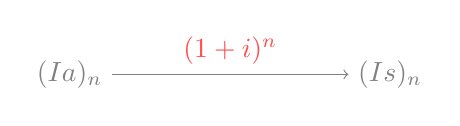
\begin{tikzpicture}
\draw [color=black!50,->](0,0) node[left]{$(Ia)_{\angles{n}}$}-- node [color=red!70,pos=0.5,above,sloped]{$(1+i)^n$}(3,0) node[right]{$(Is)_{\angles{n}}$};
    \end{tikzpicture} \\
\section{复递增年金}
$(Ca)_{\angles{n}}$:复递增年金
\begin{definition}{期末付复递增年金}
\noindent $(Ca)_{\angles{n}}=\frac{(a)_{\angles{n}}}{1+r}(r\neq i)(j=\frac{i-r}{1+r})$
\end{definition}
\begin{remark}
\noindent $(Ca)_{\angles{n}}=v+(1+r)v^2+(1+r)^2v^3+\dots+ (1+r)^{n-1}v^n$
\end{remark}